\documentclass[a4paper,11pt]{ltjsarticle}

% ========== package ========== %
% --- 数式環境 --- %
\usepackage{amsmath}
\usepackage{amssymb}
\usepackage{mathtools}
% --- 数式環境 END --- %
% ブラケット
\usepackage{braket}
% ベクトルの太文字
\usepackage{bm}
% 添え字左右上下 \fourIdx{左上}{左下}{右上}{右下}{ベース} で使う．Iは大文字
\usepackage{fouridx}
% 色
\usepackage{color}
% 余白指定
\usepackage{geometry}
% --- ページ内リンク --- %
\usepackage{hyperref}
\hypersetup{colorlinks=true,linkcolor=blue}
% --- ページ内リンク END --- %
% 花文字
\usepackage{mathrsfs}
% 画像
\usepackage{graphicx}
% tcolorbox
\usepackage{tcolorbox}
% appendix
\usepackage{appendix}
% --- 参考文献 --- %
\usepackage{etoolbox}
\usepackage{fontspec} % fontspecは読み込んでOKですが、設定順序に注意が必要です
%% --- 参考文献フォント --- %%
  \IfFontExistsTF{Times New Roman}{
    \newfontfamily\bibfontface{Times New Roman}
  }{
    \newfontfamily\bibfontface{FreeSerif} % 代替フォント
  }
%% --- 参考文献フォント END --- %%
%% --- 参考文献リンク位置 --- %%
  \BeforeBeginEnvironment{thebibliography}{%
    \phantomsection
    \addcontentsline{toc}{section}{参考文献}
  }
  \AtBeginEnvironment{thebibliography}{%
    \normalfont\bibfontface
  }
%% --- 参考文献のリンク位置 --- %%
% --- 参考文献 END --- %
% ========== package END ========== %

% ========== newcommand ========== %
% --- セクションから目次へのリンク --- %
\newcommand{\sectionlink}[1]{\section[#1]{\hyperlink{toc}{#1}}}
\newcommand{\subsectionlink}[1]{\subsection[#1]{\hyperlink{toc}{#1}}}
% セクション番号リンク
\makeatletter
\renewcommand{\@seccntformat}[1]{%
  \protect\hyperlink{toc}{\csname the#1\endcsname}\quad
}
\makeatother

\numberwithin{equation}{section}
% ==========- newcommand END ========== %
\allowdisplaybreaks
%===========================================================
% --- タイトル --- %
%===========================================================
\geometry{left=25mm, right=25mm, top=30mm, bottom=30mm}

\counterwithout{equation}{section}
\renewcommand{\theequation}{\arabic{equation}}
\renewcommand{\thetable}{\Roman{table}}
\interdisplaylinepenalty=10000
\apptocmd{\thebibliography}{\setlength{\itemsep}{-1pt}\setlength{\parsep}{0pt}}{}{}
\RenewDocumentCommand{\sectionlink}{s m}{%
  \IfBooleanTF{#1}{%
    \section*{\hyperlink{toc}{#2}}%
    \phantomsection\addcontentsline{toc}{section}{#2}%
  }{\section[#2]{\hyperlink{toc}{#2}}}%
}
\renewcommand{\abstractname}{\hyperlink{toc}{要旨}}
\newcommand{\be}{\begin{equation}}
\newcommand{\ee}{\end{equation}}
\newcommand{\bei}{\begin{itemize}}
\newcommand{\eei}{\end{itemize}}
\newcommand{\hb}{\hbar}
\newcommand{\tb}{\bar{t}}
\newcommand{\csh}{{\rm csch}}
\hypersetup{pdftitle={高周波量子ゆらぎを抑制する高温極限},pdfauthor={Graeme Pleasance, Erik Aurell, Francesco Petruccione},bookmarksnumbered=true}
\title{\bfseries 高周波量子ゆらぎを抑制する高温極限\\[0.5em]
\large\href{https://journals.aps.org/prl/abstract/10.1103/kp9j-v4ss}{High-temperature limit penalizing high-frequency quantum fluctuations}\\[0.5em]
\normalsize\href{https://arxiv.org/pdf/2508.14262v2}{arXiv:2508.14262v2 [quant-ph]}}
\author{%
Graeme Pleasance\textsuperscript{1,2}\thanks{\href{mailto:gpleasance1@gmail.com}{gpleasance1@gmail.com}},
Erik Aurell\textsuperscript{3}\thanks{\href{mailto:eaurell@kth.se}{eaurell@kth.se}},\\
Francesco Petruccione\textsuperscript{1,2,4}\thanks{\href{mailto:petruccione@sun.ac.za}{petruccione@sun.ac.za}}\\[0.6em]
\parbox{0.96\textwidth}{\centering\small
\textsuperscript{1}Department of Physics, University of Stellenbosch,\\
Stellenbosch, 7600, South Africa\\[0.25em]
\textsuperscript{2}National Institute for Theoretical and Computational Sciences\\
(NITheCS), Stellenbosch, South Africa\\[0.25em]
\textsuperscript{3}KTH -- Royal Institute of Technology, AlbaNova University Center,\\
SE-106 91 Stockholm, Sweden\\[0.25em]
\textsuperscript{4}School of Data Science and Computational Thinking,\\
University of Stellenbosch, Stellenbosch 7600, South Africa}}
\date{2026年7月9日}
\begin{document}
% 原文 main.bbl の引用順（注記2件・補足参照を含む）
\nocite{BP2002,Weiss2011,Wilner2015,Leppakangas2018,CaldeiraLeggettA,Caldeira1981,CaldeiraLeggettB,SpinBoson,Unruh1989,Zurek1993,Paz1993,ParikhWilczekZahariade2020,Kleinert2009,Breuer2001,Baym2009,FeynmanVernon,StockburgerMak1999,Stockburger1998,Stockburger2002,Diosi1993,Diosi1993a,Halliwell1995,Gao1997,Ford1999,Vacchini2000,Petruccione2005,SuppMat,Note1,Homa2019,Xu2023,Xu2025,Dekker1977,Dekker1981,Gorini1976,Lindblad1976,Note2,Aurell2020,AlickiLendi2007,Dvali2011,Hu1992,Strunz1996,DiosiStrunz1997,DiosiGisinStrunz1998,Yu2004,StrunzYu2004,DiosiFerialdi2014,Ferialdi2016,Ferialdi2017,Diosi1995}

\maketitle
\begin{abstract}
Ohmic スペクトル密度を持つ量子 Brown 運動の Caldeira-Leggett 模型を再検討し、カットオフ周波数が任意に大きい場合にも適用できる新たな高温極限において、デコヒーレンス核への付加的な寄与を導く。この寄与は、高周波量子ゆらぎの古典化をもたらす新たな機構を明らかにする。さらに、この寄与から、Lindblad 形式であることが保証された Markov 型マスター方程式が得られることを示し、このマスター方程式が量子 Brown 運動の正しい Markov 極限を記述すると論じる。本研究の方法では、浴の記憶時間のスケールで、過程の初期時刻と終時刻の両方におけるデコヒーレンス核の振る舞いを詳しく考察する。
\end{abstract}
\clearpage
\hypertarget{toc}{}
\tableofcontents
\clearpage
\sectionlink*{序論}
調和振動子からなる Ohmic 浴と相互作用する量子系の時間発展は、開放量子系の理論において最も広く研究されてきた模型の一つである\cite{BP2002}。この模型は、光子浴やフォノン浴\cite{Wilner2015}、量子回路中の抵抗素子に結合した超伝導量子ビット\cite{Leppakangas2018}など、半古典極限で減衰が摩擦のようになる\cite{Weiss2011}多くの物理的状況に適用できる。Caldeira と Leggett がこの模型を用いて量子 Brown 運動の古典極限\cite{CaldeiraLeggettA}や巨視的トンネル効果\cite{Caldeira1981,CaldeiraLeggettB}を研究したことはよく知られている。その後のスピン・ボソン問題\cite{SpinBoson}やデコヒーレンス\cite{Unruh1989,Zurek1993,Paz1993}の研究でも中心的な役割を果たし、最近では、量子化された重力子浴との相互作用によって LIGO 干渉計の腕の長さに生じる重力雑音の効果を調べるためにも用いられている\cite{ParikhWilczekZahariade2020}。

経路積分による取り扱い\cite{Kleinert2009}では、浴の影響は、相互作用のスペクトルカットオフ $\Omega$ によって記憶が制限される散逸と、さらに逆熱時間 $k_BT/\hb$ によっても記憶が制限されるデコヒーレンスに分かれる。現象論的模型やフォノン浴との相互作用では、$\Omega$ は実在の物理的パラメータである一方、光子との相互作用では正則化因子であり、繰り込みの過程で最終的に無限大にできる\cite{Breuer2001,Baym2009}。いずれの場合も、散逸は記憶を持たない。Caldeira-Leggett（CL）マスター方程式\cite{CaldeiraLeggettA}では、この散逸は系の Hamiltonian の繰り込みと二つの Lindblad 項をもたらす。後者はいずれも、位置演算子と運動量演算子の順序対 $(\hat X,\hat P)$ および $(\hat P,\hat X)$ から構成される。

これに対して、デコヒーレンスには記憶がある。熱時間 $\hb/k_BT$ が $\Omega^{-1}$ より十分長ければ、カットオフ $\Omega$ の役割は無視でき、そのまま無限大にできる。Feynman と Vernon の先駆的論文\cite{FeynmanVernon}で述べられているように、デコヒーレンスは、浴の記憶核と同じ力・力相関を持つ古典的な Gaussian 場 $\xi$ について平均することと区別できない。以上の散逸とデコヒーレンスの組み合わされた効果は、Stockburger と Mak による確率的 Liouville シミュレーション法\cite{StockburgerMak1999}の構成要素である（文献\cite{Stockburger1998,Stockburger2002}も参照）。したがって、デコヒーレンスの記憶核 $k_r$ は、調和振動子浴の影響に関する基礎的理解と、量子技術に適用される実用的なシミュレーション手法の両方で非常に重要である。同様に、熱ゆらぎを特徴づけるその役割は、高温での量子 Brown 運動の半古典的記述にとりわけ深く関わっている。

標準的な高温極限\cite{CaldeiraLeggettA}では、核 $k_r$ は記憶を持たず、位置演算子 $\hat X$ とそれ自身の順序対、すなわち $(\hat X,\hat X)$ から導かれる Lindblad 項を生成する。このとき、古典的なランダム力 $\xi$ は時間についてデルタ相関を持つ。本論文では、正しく取り扱うとマスター方程式に付加的な $(\hat P,\hat P)$ 項が現れ、それが (i) 高周波量子ゆらぎを減衰させるとともに、(ii) Born-Markov 近似と整合するパラメータのもとで系の縮約密度演算子の正値性を保つことを示す。この点は先行研究\cite{BP2002,Diosi1993,Diosi1993a,Halliwell1995,Gao1997,Ford1999,Vacchini2000,Petruccione2005}で見いだされたものと同様である。しかし本研究の導出では、$T$ を固定したまま任意に大きな（紫外）カットオフ $\Omega$ に適用できる新たな高温極限を考え、実際に $\Omega$ に全く依存しないマスター方程式が得られる。したがって、この結果は文献\cite{BP2002,Diosi1993,Diosi1993a}で導かれた類似のマスター方程式よりも広い温度範囲で有効であり、Markov 極限における中温から低温での量子 Brown 運動の研究に新たな知見を与える。

\sectionlink*{Feynman-Vernon 理論}
ポテンシャル $V(\hat X)$ 中を運動する、質量 $M$、運動量 $\hat P$、位置 $\hat X$ の量子粒子を記述する CL 模型\cite{CaldeiraLeggettA}に注目する。粒子は温度 $T$（逆温度 $\beta=1/k_BT$）にある調和振動子の熱浴と相互作用する。したがって、全 Hamiltonian は
\be\label{eq:H}
\hat{H} = \hat{H}_S + \hat{H}_B + \hat{H}_I + \hat{H}_C,
\ee
と書ける。ここで $\hat{H}_S=\hat{P}^2/2M+V(\hat{X})$ および $\hat{H}_B=\sum_k\big(\hat{p}_k^2/2m_k+\frac12m_k\omega_k^2\hat{x}_k^2\big)$ は、それぞれ系と浴の Hamiltonian である。相互作用部分には通常の双線形形式 $\hat H_I=-\hat X\otimes\sum_kc_k\hat x_k$ を採用し、$c_k$ は系と浴の結合強度を表す。最後の部分は付加的な相殺項 $\hat H_C=\hat X^2\sum_k(c_k^2/2m_k\omega_k^2)$ であり、Hamiltonian \eqref{eq:H}の並進不変性を保証する。

浴の自由度を積分消去すると、系の縮約密度演算子 $\langle X_f|\hat\rho_S(t)|X_f'\rangle$ の時間発展は、時刻 $t_i$ と $t_f$ における粒子の初期位置 $X_i$ と終位置 $X_f$ を結ぶ伝播関数 $\mathcal J(t_f,t_i)$ によって捉えられる。この伝播関数は、$X_i$ から $X_f$ への順方向経路 $X$ と、$X_i'$ から $X_f'$ への逆方向経路 $X'$ にわたる二重経路積分として表される\cite{Weiss2011}。
\be\label{eq:FV-Weiss}
\mathcal{J}(t_f,t_i) = \int\mathcal{D}X\mathcal{D}X'e^{(i/\hb)(S_S[X] - S_S[X'])}\mathcal{F}[X,X'].
\ee
ここで、$S_S[X]=\int_{t_i}^{t_f}dt\,[\frac12M\dot X^2-V(X)]$ は経路 $X(t)$ に沿った自由粒子の作用であり、$\mathcal F[X,X']$ は Feynman-Vernon（FV）影響汎関数である。浴は Gaussian 統計に従うので、影響汎関数は指数形式 $\mathcal F[X,X']=e^{-\frac{i}{\hb}S_i[X,X']-\frac1{\hb}S_r[X,X']}$ で書ける。順方向経路と逆方向経路を結合する量 $S_r[X,X']$ および $S_i[X,X']$ は、FV 作用の実部（デコヒーレンス）および虚部（散逸）を定義する。準古典的経路 $\bar X(t)=X(t)+X'(t)$ とゆらぎの経路 $\Delta X(t)=X(t)-X'(t)$\cite{Weiss2011}を用いると、これらは
\begin{align}
S_r[\Delta X] &= \int^{t_f}_{t_i}dt\int^{t}_{t_i}ds\,k_r(t-s)\Delta X(t)\Delta X(s),\label{eq:noise_action} \\
S_i[\bar{X},\Delta X] &= \int^{t_f}_{t_i}dt\int^{t}_{t_i}ds\,k_i(t-s)\Delta{X}(t)\bar{X}(s)\nonumber\\
&\qquad + \mu\int^{t_f}_{t_i}dt\,\Delta X(t)\bar{X}(t),
\end{align}
と書ける。$\mu=\sum_kc_k^2/(2m_k\omega_k^2)$ は浴の再配置エネルギーである（$\mu\sim\Omega$）。核 $k_r$ と $k_i$ は、浴の相関関数 $k(\tau)=\sum_k(c_k^2/2m_k\omega_k)[\coth(\hb\omega_k/2k_BT)\cos(\omega_k\tau)-i\sin(\omega_k\tau)]$ の実部と虚部を表す。実部、すなわち FV 核\cite{FeynmanVernon}は、非対角経路 $\Delta X(t)$ に沿った量子ゆらぎの減衰を支配する。FV 影響汎関数の中では、記憶時間 $\tau_B$ を持つ Gaussian 確率力の力・力相関関数の役割を果たす［後述の式\eqref{eq:FV_trick}を参照］。Ohmic スペクトル密度 $J(\omega)=2\eta\omega\theta(\Omega-\omega)$ を持つ浴では、$J(\omega)=\frac\pi2\sum_k(c_k^2/m_k\omega_k)\delta(\omega-\omega_k)$ とすると、FV 核は
\be\label{eq:FV}
k_r(\tau) = \frac{2\eta}{\pi}\int^{\Omega}_0d\omega\,\omega\coth{\left(\frac{\hb\omega}{2k_BT}\right)}\cos{\omega\tau}.
\ee
となる。$k_r$ の白色雑音極限が高温で実現されることはよく知られている\cite{CaldeiraLeggettA}。具体的に、$\tau_B=\hb/k_BT$ とする。$\tau_B\to0$ の極限で $\coth(\hb\beta\omega/2)\approx2/\hb\beta\omega$ と近似すると、粒子が $\Omega^{-1}$ より十分長い時間スケールで発展する限り、特異な核 $k_r^{(0)}(\tau)=(4\eta/\tau_B)\delta(\tau)$ が得られる。

\begin{figure}[tbp]
\centering
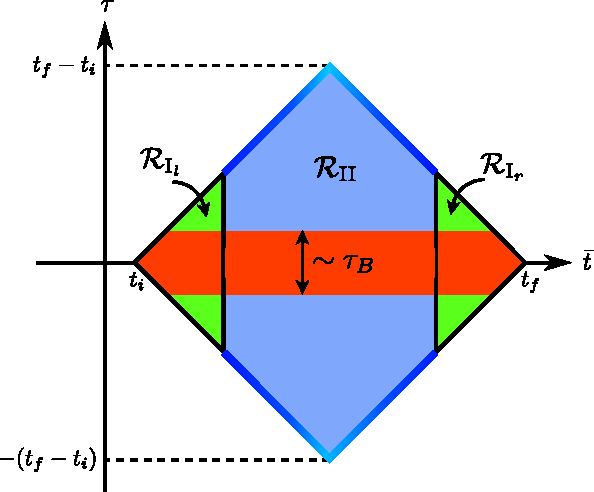
\includegraphics[width=0.72\textwidth]{source/fig1.pdf}
\caption{式\eqref{eq:decoh_action}の積分領域全体と、その部分領域 $\mathcal R_{\rm I}=\mathcal R_{{\rm I}_l}\cup\mathcal R_{{\rm I}_r}$ および $\mathcal R_{\rm II}$ を示す模式図。$\tau\gg\tau_B$ となる赤色領域の外側では核は実質的にゼロなので、$|t_f-t_i|\gg\tau_B$ を仮定すると、青色領域の $\tau$ 積分の限界を $\pm\infty$ まで拡張できる。緑色領域は、積分限界を無限大にできない端点寄与の台を示す。三つの部分領域すべての境界を示した、より詳細な図を文献\cite{SuppMat}に示す。}
\label{fig1}
\end{figure}

\sectionlink*{Feynman-Vernon 核とデコヒーレンス作用}
次に、FV 核がデコヒーレンス作用に非特異な寄与を与える新たな高温極限を導く。以下に示すように、これによって CL マスター方程式に拡散型の項が付加され、高周波量子ゆらぎを減衰させる。本論文を通じた方針は、FV 核を緩増加超関数 $k_r\in\mathcal S'(\mathbb R)$\cite{Note1}として扱うことである。対応する試験関数は $\mathcal S(\mathbb R)$ に属し、$\Omega^{-1}$ より短い時間スケールでの変動は無視できるとあらかじめ仮定する。この目的のために、FV 核の次の表示を用いると便利である\cite{SuppMat}。
\be\label{eq:kern_func}
k_r(\tau) = \frac{2\eta}{\pi}\left[-\frac{\pi^2}{\tau_B^2}\csh^2(\pi\tau/\tau_B)+\Omega^2\,O\left(\frac{1}{(\Omega\tau)^3}\right)\right].
\ee
この式から、$k_r$ の振る舞いには二つの領域があることがわかる。
\bei
\item[(i)] 真空領域 $\Omega^{-1}\ll\tau\ll\tau_B$：漸近展開 $\csh^2x=\frac1{x^2}-\frac13+O(x^2)$ を用いると、式\eqref{eq:kern_func}は
\be\label{eq:kern_short_time}
k_r(\tau)\approx-\frac{2\eta}{\pi}\frac1{\tau^2},
\ee
と近似できる。これは、$k_r(\tau)$ の短時間の振る舞いが真空寄与 $k_r^{\rm vac}(\tau)=\frac{2\eta}{\pi}\int_0^\Omega d\omega\,\omega\cos\omega\tau$ に支配されることを意味する。特に、
\be
k_r^{\rm vac}(\tau)=\frac{2\eta}{\pi}\left[-\frac1{\tau^2}+\Omega^2O\left(\frac1{(\Omega\tau)^3}\right)\right].
\ee
\item[(ii)] 指数関数的領域 $\tau\gg\tau_B\gg\Omega^{-1}$：$x\gg1$ に対して $\csh^2x\sim e^{-2x}$ となることを用いると、
\be\label{eq:kern_exp_long_time}
k_r(\tau)\approx-\frac{2\eta}{\pi}\frac1{\tau_B^2}e^{-2|\tau|/\tau_B}.
\ee
\eei
これらの関係から、核\eqref{eq:FV}は $\tau>0$ に対してスケーリング極限 $\Omega\to\infty$ で収束し、浴の逆温度によって定まる時刻 $|\tau|\gtrsim\tau_B$ を超えると消失することがわかる。

デコヒーレンス汎関数\eqref{eq:noise_action}を評価するため、まず新たな変数 $\tb=\frac12(t+s)$ および $\tau=t-s$ を用いて二重積分を書き直す。
\be\label{eq:decoh_action}
S_r[\Delta X]=\frac12\iint_{\mathcal R}d\tb\,d\tau\,k_r(\tau)\Delta X(\tb+\tau/2)\Delta X(\tb-\tau/2).
\ee
$(\tb,\tau)$ 平面内の積分領域 $\mathcal R$ を図\ref{fig1}に示す。これは、$\mathcal R_{{\rm I}_l}$（左）、$\mathcal R_{{\rm I}_r}$（右）、$\mathcal R_{\rm II}$ の三つの部分領域からなり、最初の二つはデコヒーレンス作用への端点項の寄与を表す。解析を簡単にするため、ここでは端点項を除いて $S_r[\Delta X]$ を評価する。これらの項の役割は高温で無視できることを示せる。端点寄与を明示的に扱うより詳細な解析は、補足資料\cite{SuppMat}の第 III 節に示す。以下では、デコヒーレンス作用を
\begin{equation}\label{eq:decoh_func}
S_r[x]\approx\frac\eta\pi\frac1{\tau_B}\int_{t_i}^{t_f}d\tb\int_{-\infty}^{\infty}ds\,F_{\Omega\tau_B}(s)x_{\tb}(s),
\end{equation}
と近似する。ここで、$x_{\tb}(s)=\Delta X(\tb+\tau_Bs/2)\Delta X(\tb-\tau_Bs/2)$、$F_\Lambda(s)=\int_0^\Lambda ds\,x\coth\frac x2\cos sx$ である。

$F_\Lambda$ が緩増加であることから許される部分積分を式\eqref{eq:decoh_func}に繰り返し適用することで、上式の内側の積分を二群の項、すなわち式\eqref{eq:kern_func}で与えられる FV 核の主要寄与に依存する項と、高次の寄与に依存する境界項に分離できる。特に、後者はスケーリング極限 $\Omega\to\infty$ で消失することが示される（補足資料\cite{SuppMat}の第 II 節を参照）。そこで主要な項だけを残し、記憶核を $k_r^{(m)}(\tau)=(\pi^2/\tau_B^2)\csh^2(\pi\tau/\tau_B)$ と定義すると、デコヒーレンス作用は次の二つの汎関数の和として表せる。
\begin{align}\label{eq:action}
S_r[\Delta X]&:=S_r^{(0)}[\Delta X]+S_r^{(m)}[\Delta X]\nonumber\\
&=\frac{2\eta}{\pi}\int_{t_i}^{t_f}dt\bigg[\frac\pi{\tau_B}\Delta X^2(t)\nonumber\\
&\quad+\int_0^\infty d\tau\,k_r^{(m)}(\tau)\big(\Delta X^2(t)-\Delta X(t+\tau/2)\Delta X(t-\tau/2)\big)\bigg].
\end{align}
最初の汎関数 $S_r^{(0)}[\Delta X]$ は、記憶のない核 $k_r^{(0)}$ を用いてデコヒーレンス作用に対して得られる標準的な高温の結果と等価である。さらに興味深いのは、$k_r^{(m)}$ に依存する二番目の汎関数 $S_r^{(m)}[\Delta X]$ が白色雑音極限の外側でも有効であり、したがって短時間の記憶効果を取り入れたデコヒーレンス作用への寄与を表すことである。このことは、$\tau_B\to0$ のとき $S_r^{(m)}[\Delta X]$ が消失することに示されている。これは、内側の括弧内にある経路の差を $\tau$ の最低次まで展開すれば直接わかる。したがって、ゆらぎの経路の展開に高次の項を含めることで、白色雑音作用 $S_r^{(0)}[\Delta X]$ への補正を系統的に導ける。

\begin{table}[tbp]
\centering
\resizebox{\textwidth}{!}{%
\begin{tabular}{cccccc}
\hline\hline
マスター方程式 & パラメータ & Lindblad 形式 & $D_{XX}$ & $D_{PP}$ & $D_{XP}$\\\hline
\textbf{本研究} & $\hb\gamma\ll k_BT\ll\hb\Omega$ & はい & $\frac{\gamma}{6Mk_BT}$ & $\frac{2\gamma Mk_BT}{\hb^2}$\rule{0pt}{3ex} & $0$\\[1ex]
Di\'{o}si\cite{Diosi1993,Diosi1993a} & $\hb\gamma\ll\hb\Omega\leq k_BT$ & はい & $\frac{\gamma}{6Mk_BT}$ & $\frac{2\gamma Mk_BT}{\hb^2}$ & $\frac{\Omega\gamma}{6\pi k_BT}$\\[1.5ex]
Breuer-Petruccione\cite{BP2002} & $\hb\gamma\ll\hb\Omega\leq k_BT$ & はい & $\frac{\gamma}{8Mk_BT}$ & $\frac{2\gamma Mk_BT}{\hb^2}$ & $-\frac{\gamma k_BT}{\hb^2\Omega}$\\[1.5ex]
Caldeira-Leggett\cite{CaldeiraLeggettA} & $\hb\gamma\ll\hb\Omega\leq k_BT$ & いいえ & $0$ & $\frac{2\gamma Mk_BT}{\hb^2}$ & $0$\\[1ex]
\hline\hline
\end{tabular}}
\caption{\label{tab1}高温極限で導かれた種々の Markov 型マスター方程式と、それぞれの拡散係数の比較\cite{Homa2019}。文献\cite{Diosi1993,Diosi1993a}では、特定のパラメータ極限で CL マスター方程式が Lindblad 形式として再導出されている。また、文献\cite{BP2002}の式 (3.409) で導かれた交差拡散項 $D_{PX}$ は、系の発展が $\Omega^{-1}$ に比べて遅い場合には $D_{PP}$ に比べて無視できるものとして扱われている。}
\end{table}

\sectionlink*{新たな高温極限}
次に、$x_t(s)$ を $\tau_Bs$（または $\tau$）の次の主要次数まで展開する。
\be\label{eq:x_expand}
x_t(s)=x_t^{(0)}+(\tau_Bs)^2x_t^{(1)}+\ldots,
\ee
ここで $x_t^{(0)}=\Delta X_t^2$ であり、式\eqref{eq:action}は
\begin{equation}\label{eq:action_exp}
S_r[\Delta X]=S_r^{(0)}[\Delta X]+S_r^{(1)}[\Delta X]+\ldots,
\end{equation}
となる。ただし、
\begin{align}\label{eq:decoh_action_1}
S_r^{(1)}[\Delta X]&:=\frac{\eta\tau_B}{6}\int_{t_i}^{t_f}dt\,\Delta X(t)\left(-\frac{\partial^2}{\partial t^2}\right)\Delta X(t)\\
&\quad+\text{（境界項）}.\nonumber
\end{align}
ここでは $\int_0^\infty d\tau/\tau_B\,\tau^2k_r^{(m)}(\tau)=\pi/6$ を用いた。式\eqref{eq:decoh_action_1}は本論文の第一の結果であり、白色雑音作用に対する主要な高温補正を与える。平均ゼロ $\mathbb E[\xi(t)]=0$、相関 $\mathbb E[\xi(t)\xi(s)]=k_r^{\rm eff}(t-s)$ の補助 Gaussian 場 $\xi(t)$ に関する平均として $\exp(-S_r[\Delta X]/\hb)$ を書き直すことで、汎関数\eqref{eq:decoh_action}におけるその役割を明らかにできる。このため、$\lambda=2\sqrt3/\tau_B$、$\sigma=\sqrt{3/\eta\tau_B}$ として微分演算子 $K(t)=\frac1{\sigma^2}\big(-\frac{\partial^2}{\partial t^2}+\lambda^2\big)$ を導入する。すると、式\eqref{eq:action_exp}の主要な補正までで $\exp(-S_r[\Delta X]/\hb)=\exp(-\frac1{2\hb}\int_{t_i}^{t_f}dt\,\Delta X(t)K[\Delta X](t))$ となる。この指数関数は、Hubbard-Stratonovich 変換によって次のように書き換えられる\cite{StockburgerMak1999,Xu2023,Xu2025}。
\begin{align}\label{eq:FV_trick}
&\exp(-S_r[\Delta X]/\hb)=\text{（自明な因子）}\nonumber\\
&\quad\times\int\mathcal D\xi\,P[\xi]\exp\left(-\frac i{\hb}\int_{t_i}^{t_f}dt\,\xi(t)\Delta X(t)\right),
\end{align}
ここで $P[\xi]=N^{-1}\exp(-\frac1{2\hb}\int_{t_i}^{t_f}dt\,\xi(t)K^{-1}[\xi](t))$ は Gaussian 確率汎関数である。この式の自明な前置因子は、式\eqref{eq:decoh_action_1}の境界項に由来する。また、$K^{-1}[\xi]=\int_{t_i}^{t_f}ds\,G(t-s)\xi(s)$ であり、$G(t-s)$ は演算子 $K(t)$ の（対称な）Green 関数である。

この核は正定値であり、$\frac1{\sigma^2}\big(-\frac{\partial^2}{\partial t^2}+\lambda^2\big)G(t-s)=\delta(t-s)$ を満たす必要があるので、$k_r^{\rm eff}(t-s)=K(t-s)\delta(t-s)$ を容易に導ける。注目すべきことに、この力・力相関関数は、高温極限で次の主要項まで展開した FV 核、すなわち $k_r(\tau)\approx\frac{4\eta}{\tau_B}\delta(\tau)-\frac{\eta\tau_B}{3}\delta''(\tau)$ と等価である。したがって、補正項 $S_r^{(1)}[\Delta X]$ は、FV 核を $O(\hb\beta)$ まで扱うことで類似の補正を導いた Di\'{o}si\cite{Diosi1993,Diosi1993a}と同じ近似水準で有効である。そこでの補正は CL マスター方程式に拡散項を付加し、Lindblad 形式にすることが示されていた\cite{Diosi1993,Diosi1993a}。同様に、本研究の結果からも Lindblad 形式のマスター方程式が得られるが、その Dekker 係数\cite{Dekker1977,Dekker1981}はカットオフ $\Omega$ に依存しないことを示す。

\sectionlink*{Feynman-Vernon 核からの Lindblad マスター方程式の導出}
完全正で一様連続な力学的半群を生成する Liouville 演算子 $\mathcal L$ の最も一般的な表現は、Lindblad 形式である\cite{Gorini1976,Lindblad1976}。
\begin{align}\label{eq:me}
\frac{\partial\hat\rho_S(t)}{\partial t}&=\mathcal L\hat\rho_S(t)\nonumber\\
&=-\frac i{\hb}[\hat H_{\rm eff},\hat\rho_S]+\sum_{i,j}a_{ij}\Big(\hat L_i\hat\rho_S\hat L_j^\dagger-\frac12\{\hat\rho_S,\hat L_j^\dagger\hat L_i\}\Big),
\end{align}
ここで、$\hat L_i$ は Lindblad 演算子、$\hat H_{\rm eff}$ は Hamiltonian である\cite{Note2}。行列 $\boldsymbol a$ が必ず半正定値、$\boldsymbol a\succeq0$ であることにより、この方程式から得られる解の正値性が保証される。文献\cite{BP2002,CaldeiraLeggettA}で Born-Markov 近似のもとに導かれた CL マスター方程式は、Lindblad 演算子 $\hat L_1=\hat X$、$\hat L_2=\hat P$ と Kossakowski 行列
\be\label{eq:a0}
\boldsymbol a_0=\begin{pmatrix}
4\gamma Mk_BT/\hb^2&-i\gamma/\hb\\
i\gamma/\hb&0
\end{pmatrix},\qquad\gamma=\eta/M
\ee
を持ち、式\eqref{eq:me}と同じ形になる。この行列のスペクトルは常に負の固有値を含む（$\det\boldsymbol a_0<0$）。この不整合の理由は、FV 核の高温展開における次の主要寄与から現れる $(\hat P,\hat P)$ 項が欠けていることにある\cite{BP2002,Diosi1993,Diosi1993a,Gao1997,Ford1999,Vacchini2000}。本研究では、FV 影響汎関数を超演算子表示\cite{Aurell2020}で書き直すと、Liouville 演算子
\begin{align}\label{eq:liouville}
\mathcal L\hat\rho_S&=-\frac i{\hb}[\hat H_S,\hat\rho_S]-i\frac\gamma{\hb}[\hat X,\{\hat P,\hat\rho_S\}]-D_{PP}[\hat X,[\hat X,\hat\rho_S]]\nonumber\\
&\quad-D_{XX}[\hat P,[\hat P,\hat\rho_S]]-2D_{XP}[\hat X,[\hat P,\hat\rho_S]],
\end{align}
が得られる。ここで、
\be\label{eq:dc}
D_{XX}=\frac\gamma{6Mk_BT},\qquad D_{PP}=\frac{2\gamma Mk_BT}{\hb^2},\qquad D_{XP}=0,
\ee
は現象論的な Dekker 係数である\cite{Dekker1977,Dekker1981}。式\eqref{eq:liouville}は $\hat H_S$ に含まれるポテンシャル $V(\hat X)$ の形によらず成立する。ポテンシャルは粒子の自由発展のみに影響し、拡散時間スケール\eqref{eq:dc}には影響しない\cite{AlickiLendi2007}。$\hat L_1=\hat X$、$\hat L_2=\hat P$ とすると、Liouville 演算子\eqref{eq:liouville}から得られる Kossakowski 行列が、$\det\boldsymbol a=4D_{XX}D_{PP}-\frac{\gamma^2}{\hb^2}\geq0$ によって正値性の制約を満たすことを容易に示せる。したがって、位置拡散係数 $D_{XX}$ は、マスター方程式を常に Lindblad 形式にするのに十分大きい。また、付加的な $(\hat P,\hat P)$ 項は高周波量子ゆらぎを減衰させるので、十分な高周波では、浴と相互作用する量子系は古典的に振る舞う。これは、開放量子系における\textit{古典化}への新たな道筋である\cite{Dvali2011}。

表\ref{tab1}は、本研究で導かれた Markov 型マスター方程式［式\eqref{eq:liouville}--\eqref{eq:dc}］と、文献\cite{Diosi1993,Diosi1993a,CaldeiraLeggettA,BP2002}で導かれたものの主な違いをまとめたものである。

\sectionlink*{厳密なマスター方程式との関係}
最後に、$\hat L_1=\hat X$、$\hat L_2=\hat P$、$\hat H_{\rm eff}=\hat P^2/2M+\frac12M\omega_0^2\hat X^2$ とした式\eqref{eq:me}は、非 Markov 型量子 Brown 運動を記述する厳密な Hu-Paz-Zhang（HPZ）マスター方程式\cite{Hu1992}とは本質的に異なる構造を持つことを指摘する（類似の厳密な結果については文献\cite{Strunz1996,DiosiStrunz1997,DiosiGisinStrunz1998,Yu2004,StrunzYu2004,DiosiFerialdi2014,Ferialdi2016}も参照）。その原因は、HPZ マスター方程式に直接の対応物を持たない $(\hat P,\hat P)$ 項にある。文献\cite{Ferialdi2016,Ferialdi2017}では、この違いは散逸が CL 模型に本来備わる非 Markov 的な特徴であることに由来し、Markov 極限で散逸を取り入れるには、運動量を介した浴との結合を導入する必要があると論じられた\cite{Diosi1995,Halliwell1995,Gao1997,Vacchini2000}。特に、外部雑音への位置結合と運動量結合の両方を含む現象論的な方法は、時間局所的なマスター方程式\cite{Ferialdi2016}
\begin{align}\label{eq:tl_liouvillian}
\mathcal L_t\hat\rho_S&=-i[\hat H_{\rm eff}(t),\hat\rho_S]+\Gamma(t)[\hat X,[\hat X,\hat\rho_S]]+\Theta(t)[\hat X,[\hat P,\hat\rho_S]]\nonumber\\
&\quad+\Xi(t)[\hat X^2,\hat\rho_S]+\Upsilon(t)[\hat X,\{\hat P,\hat\rho_S\}]+\gamma(t)[\hat P,[\hat P,\hat\rho_S]]
\end{align}
の確率過程による表示を与えることが示されており、ここには $(\hat P,\hat P)$ 項が実際に現れる。式\eqref{eq:tl_liouvillian}は白色雑音極限で式\eqref{eq:liouville}に帰着するので、Markov 領域の量子 Brown 運動を正しく記述するには $\hat P$ 結合が必要であると結論された。

これに対して我々は、Markov 型量子 Brown 運動は本論文で導入した新たな高温極限のもとで最も適切に記述されると考える。その根拠は、表\ref{tab1}に挙げた他のマスター方程式では、Markov 極限 $\Omega\to\infty$ をとるために $T\to\infty$ も必要であり、これは FV 核の主要寄与 $k_r\sim\delta(\tau)$ だけを残すことに相当するという事実にある。この種の核は、力学の完全正値性が失われる非物理的な記述をもたらす。しかし本研究の方法では、真に記憶のない浴 $\Omega\to\infty$ を課すと同時に、$k_r$ の次の主要寄与を残すことができ、これが Markov 極限の正しい実行方法であることを示唆している。結局、調和ポテンシャル $V(\hat X)=\frac12M\omega_0^2\hat X^2$ を持つ式\eqref{eq:liouville}は、HPZ マスター方程式\cite{BP2002}の極限としては得ることが\textit{できず}、この点で本研究の結果は文献\cite{Hu1992,StrunzYu2004,Yu2004}と区別される。

また、式\eqref{eq:liouville}は次の確率的 Schr\"odinger 方程式による表示を持つ\cite{StrunzYu2004}。
\begin{equation}
\dot\psi_t=\Big(-\frac i\hbar\hat H_S+\sum_i\hat L_i\phi_i(t)-\frac12\sum_{i,j}a_{ij}\hat L_j^\dagger\hat L_i\Big)\psi_t,
\end{equation}
ここで $\phi_i(t)$ は平均ゼロの Gaussian 白色雑音であり、$\mathbb E[\phi_i(t)\phi_j^*(s)]=a_{ij}\delta(t-s)$、$\mathbb E[\phi_i(t)\phi_j(s)]=0$ である。この方程式には、文献\cite{Ferialdi2016}で現象論的に導入されたものと同様の、運動量と雑音の結合項 $\hat P\phi(t)$ が含まれる。したがって、FV 核の次の主要項 $\sim\delta''(\tau)$ を含めれば、文献\cite{Halliwell1995,Gao1997,Ford1999,Vacchini2000,Petruccione2005,Diosi1995}と整合して完全正値性を保つために必要な有効な $\hat P$ 結合を導入するのに十分である。

\sectionlink*{結論}
本論文では、調和振動子からなる Ohmic 浴と相互作用する量子粒子を記述する CL 模型の新たな高温極限を導いた。この極限における系の縮約力学は Lindblad 形式の Markov 型マスター方程式によって捉えられることが示された。これは、量子 Brown 運動の従来の白色雑音による取り扱いで用いられる CL マスター方程式\cite{CaldeiraLeggettA}や、その他の類似の研究\cite{Diosi1993,Diosi1993a,Halliwell1995,Gao1997,Ford1999,Vacchini2000,Petruccione2005}とは異なる。

さらに、マスター方程式\eqref{eq:liouville}は任意の形のポテンシャル $V(\hat X)$ に適用でき、完全正な量子 Brown 運動を記述するために、浴との運動量結合を別途加える必要がない。この結果は紫外カットオフ $\Omega$ を持つ浴にも適用できるので、Born-Markov 近似 $\hb\gamma\ll k_BT$ を満たす程度に温度がなお十分高ければ、文献\cite{BP2002,CaldeiraLeggettA,Diosi1993}で規定された温度領域の外でも適用可能であると考えられる（表\ref{tab1}を比較）。これらのマスター方程式をより形式的に比較するには、調和振動子系について、それぞれの予測を厳密な HPZ マスター方程式\cite{Hu1992}と比較して検証する方法が考えられる。また、ゆらぎの経路の展開\eqref{eq:x_expand}に高次の項を含めることで、本研究の結果をより低い温度領域へ系統的に拡張できる可能性があるが、これは今後の課題とする。

\clearpage
\renewcommand{\refname}{\hyperlink{toc}{参考文献}}
\bibliographystyle{utphys}
\bibliography{ref}
\clearpage
\sectionlink*{「高周波量子ゆらぎを抑制する高温極限」の補足資料}
\begin{center}
Graeme Pleasance, Erik Aurell, Francesco Petruccione
\end{center}
\sectionlink*{I. Feynman-Vernon 核の導出}

本節では、本文の式\eqref{eq:kern_func}に示した FV 核の導出を概説する。この方法は、Ohmic 浴と相互作用する相対論的粒子のデコヒーレンス汎関数を評価するために文献\cite{BP2002}で示された導出［同文献の式 (12.172) を参照］に部分的に基づいており、完全を期すため、ここにその全体を再掲する。

まず、次の関数を定義する。
\be\label{eq:F}
    F_{\Lambda}(s) = \int^{\Lambda}_0dx\,x\coth\frac{x}{2}\cos{sx},
\ee
これは FV 核と次の関係にある（$\tau_B = \hb\beta$）。
\begin{align}\label{eq:fv_kern}
	k_r(\tau) &= \frac{2\eta}{\pi}\Big(\frac{1}{\hb\beta}\Big)^2\int^{\Omega\hb\beta}_0dx\,x\coth\frac{x}{2}\cos\frac{x\tau}{\hb\beta} \nonumber\\
		 &= \frac{2\eta}{\pi}\frac{1}{\tau_B^2} F_{\Omega\tau_B}(\tau/\tau_B).
\end{align}
さらに、式\eqref{eq:F}の1階および2階の原始関数を導入する。
\begin{align}
	G_{\Lambda}(s) &= \int^{\Lambda}_0dx\,\coth\frac{x}{2}\sin sx, \\
	H_{\Lambda}(s) &= \int^{\Lambda}_0dx\,\coth\frac{x}{2}\left(\frac{1-\cos sx}{x}\right),
\end{align}
これらは
\be\label{eq:primatives}
	\frac{d^2}{ds^2}H_{\Lambda}(s) = \frac{d}{ds}G_{\Lambda}(s) = F_{\Lambda}(s),
\ee
を満たす。また、$H_{\Lambda}(s)$ を真空部分 $H^{\rm vac}_{\Lambda}(s)$ と熱的部分 $H^{\rm th}_{\Lambda}(s)$ に分ける\cite{BP2002}。
\begin{align}
	H_{\Lambda}(s) &:= H^{\rm vac}_{\Lambda}(s) + H^{\rm th}_{\Lambda}(s) \nonumber\\
    &= \int^{\Lambda}_0dx\frac{1-\cos sx}{x} + \int^{\Lambda}_0dx\left(\coth\frac{x}{2}-1\right)\frac{1-\cos sx}{x}.
\end{align}
ここで、真空の寄与については
\begin{align}\label{eq:H_vac}
	H^{\rm vac}_{\Lambda}(s) &= \int^{\Lambda s}_0dx\frac{1-\cos x}{x} \nonumber\\
					  &= {\rm ln}\,g\Lambda s + \int^{\infty}_{\Lambda s}dx\frac{\cos x}{x} = {\rm ln}\,g\Lambda s + O\left(\frac{1}{\Lambda s}\right),
\end{align}
となる。2番目の等号では恒等式 $\int^{\infty}_{\Lambda s}dx\frac{\cos x}{x} = -\ln g\Lambda s + \int^{\Lambda s}_0dx\frac{1-\cos x}{x}$ を用い、$\ln g\approx 0.577$ は Euler-Mascheroni 定数である。式 (\ref{eq:H_vac}) を微分すると、真空の項としてさらに
\begin{align}
	G^{\rm vac}_{\Lambda}(s) &= \frac{1}{s} + \Lambda \,O\left(\frac{1}{(\Lambda s)^2}\right) \\
	F^{\rm vac}_{\Lambda}(s) &=  -\frac{1}{s^2} + \Lambda^2\,O\left(\frac{1}{(\Lambda s)^3}\right).
\end{align}
を得る。$G_{\Lambda}(s)$ の熱的成分
\be
	G^{\rm th}_{\Lambda}(s) = \int^{\Lambda}_0dx\left(\coth\frac{x}{2} -1\right)\sin sx,
\ee
については、$x>1$ で $(\coth\frac{x}{2}-1)$ が指数関数的に減衰するため、積分の上限を無限大まで拡張できる。したがって、恒等式
\[
	\coth\frac{x}{2} -1 = 2\sum^{\infty}_{n=0}e^{-(n+1)x}
\]
から
\begin{align}\label{eq:G_therm}
	G^{\rm th}_{\Lambda}(s) &\approx 2\,{\rm Im}\int^{\infty}_0dx\sum^{\infty}_{n=0}e^{isx - (n+1)x} \nonumber\\
    &= \pi\coth \pi s - \frac{1}{s},
\end{align}
となる。ここで2番目の等号は Matsubara 分解
\[
	\coth\frac{x}{2} = 2\left(\frac{1}{x} + 2\sum^{\infty}_{n=1}\frac{x}{x^2+(2\pi n)^2}\right).
\]
から得られる。次に、$G^{\rm vac}_{\Lambda}(s)$ と式\eqref{eq:G_therm}を組み合わせると
\be\label{eq:G}
	G_{\Lambda}(s) = \pi\coth\pi s + \Lambda O\left(\frac{1}{(\Lambda s)^2}\right).
\ee
を得る。$F_{\Lambda}(s)$ の熱的部分も、式 (\ref{eq:G}) を微分することによって
\be
	F^{\rm th}_{\Lambda}(s) = -\frac{\pi^2}{\sinh^2\pi s} + \frac{1}{s^2},
\ee
と求められる。したがって、$F_{\Lambda}(s)$ の真空部分と熱的部分を組み合わせると
\be\label{eq:FL}
	F_{\Lambda}(s) = -\pi^2\csh^2\pi s + \Lambda^2O\left(\frac{1}{(\Lambda s)^3}\right).
\ee
となる。式\eqref{eq:fv_kern}に戻ると、FV 核は
\be
	k_r(\tau) =  \frac{2\eta}{\pi}\left[-\frac{\pi^2}{\tau_B^2}\csh^2(\pi \tau/\tau_B) + \Omega^2\,O\left(\frac{1}{(\Omega \tau)^3}\right)\right].
\ee
と与えられる。

\sectionlink*{II. デコヒーレンス汎関数の評価}\label{sec:functional}

本節では、端点項の寄与を除いた、本文の式\eqref{eq:action}に示すデコヒーレンス汎関数の具体的な形を導出する。出発点として、汎関数 $T_F:\mathcal{S}(\mathbb{R})\rightarrow\mathbb{R}$ を導入する。
\be\label{eq:functional}
T_F[x_{\tb}] = \int^{\infty}_{-\infty}ds\,F_{\Lambda}(s)x_{\tb}(s),
\ee
これは、揺らぎの経路 $x_{\tb}(s)=\Delta X(\tb+\tau_Bs/2)\Delta X(\tb - \tau_Bs/2)$ の集合を含む試験関数の空間 $\mathcal{S}(\mathbb{R})$ に作用する。本文で述べたように、これらの経路は $\Omega^{-1}$ よりも短い時間スケールでは変化が無視できるものと仮定する。積分\eqref{eq:functional}を、パラメータ $q$ で定まる互いに重ならない3つの部分区間に分割する（図\ref{fig2}を参照）。
\be\label{eq:functional_supp}
T_F[x] = \int^{q}_{-q}ds\,F_{\Lambda}(s)x(s) + \int^{\infty}_qds\,F_{\Lambda}(s)x(s) + \int^{-q}_{-\infty}ds\,F_{\Lambda}(s)x(s),
\ee
ここで、表記を簡単にするため $x_{\tb}$ の添字を省略した（以後、特に断らない限り、$x_{\tb}$ の $\tb$ 依存性は明示しない）。$x(s)=x(0)+O(s)$ と展開すると、最初の積分は
\begin{align}\label{eq:func_q}
    \int^q_{-q}ds\,F_{\Lambda}(s)x(s) &= \int^{\Lambda}_0dy\,y\coth\frac{y}{2}\bigg(\int^{q}_{-q}ds\,x(s)\cos{sy}\bigg) \nonumber\\
    &= x(0)\int^{\Lambda}_0dy\,y\coth\frac{y}{2}\bigg(\int^q_{-q}ds\,\cos{sy}\bigg) + ... \nonumber\\
    &= 2G_{\Lambda}(q)x(0) + ... \, .
\end{align}
と書ける。ここで $\Lambda q\gg1$ と仮定すると、式\eqref{eq:G}および\eqref{eq:func_q}の主要項を用いて、十分に小さい $q$ に対し、分布 $F_{\Lambda}(s)$ が区間 $[-q,q]$ 上で Dirac のデルタ関数のように振る舞うことが分かる。
\[
    x\mapsto \int^q_{-q}ds\,F_{\Lambda}(s)x(s)= 2\pi\coth{(\pi q)}x(0),\qquad q\gg\Lambda^{-1}.
\]
そこで、式\eqref{eq:FL}を用いて次のようにも書ける。
\be
    T_F[x] = 2\pi\int^q_{-q}ds\,x(s)\delta(s)\coth{(\pi q)} - \pi^2\bigg[\int^{\infty}_qds\,x(s)\csh^2{(\pi s)} + \int^{-q}_{-\infty}ds\,x(s)\csh^2{(\pi s)}\bigg],
\ee
角括弧内の項を部分積分すると
\begin{align}
    T_F[x] &= 2\pi\coth{(\pi q)}\int^q_{-q}ds\,x(s)[\delta(s) - \delta(s+q) - \delta(s-q)] \nonumber\\
    &\qquad - \pi\int^{\infty}_qds\,\coth{(\pi s)}[x'(s) - x'(-s)].
\end{align}
となる。さらに上式の2行目に部分積分を2回適用すると
\be\label{eq:functional_ibp}
    T_F[x] = 2\pi\,\coth{(\pi q)}[x(0) - x(q)] - 2\pi\int^{\infty}_qds\,\coth{(\pi s)}\,x'(s),
\ee
を得る。ここでは $x(s)$ が偶関数であることを用いた。残りの積分を評価するため、導関数 $x'(s)$ を
\be\label{eq:deriv}
    x'(s) = \frac{d}{ds}[x(s) - x(0)].
\ee
と書く。$x'(s)$ をこの形にする必要があるのは、そうしなければ結果に発散する項が生じるためである（$\coth{(\pi s)}$ は原点で可積分ではない）。したがって、式\eqref{eq:functional_ibp}の第2項を部分積分すると
\be
    T_F[x] =  2\pi\bigg(x(0) - \pi\int^{\infty}_qds\,\csh^2{(\pi s)}[x(s) - x(0)]\bigg).
\ee
となる。次に $q\rightarrow 0$ の極限を取る。この極限は、同時に $\Lambda\rightarrow \infty$（$\Omega\rightarrow\infty$）として $\Lambda q \gg 1$ を保証することで正当化される（例えば $q\sim \Lambda^{-\alpha}$、$0<\alpha<1$ と固定することで制御できる）。すると
\be\label{eq:T_lim}
    \lim_{\Lambda\rightarrow\infty}\lim_{q\rightarrow 0}T_F[x_{\tb}] =  2\pi\bigg(x_{\tb}(0) - \pi\int^{\infty}_0ds\,\csh^2(\pi s)[x_{\tb}(s) - x_{\tb}(0)]\bigg),
\ee
を得る。ここで $x$ に添字 $\tb$ を再び付けた。導関数\eqref{eq:deriv}が原点でゼロになるため、この極限で積分は収束することに注意されたい。最後に
\be
    S_r[x] = \frac{\eta}{\pi}\frac{1}{\tau_B}\int^{t_f}_{t_i}d\tb\,T_F[x_{\tb}]
\ee
を用い、式\eqref{eq:T_lim}を代入すると、本文の式\eqref{eq:action}が得られる。

\sectionlink*{III. デコヒーレンス汎関数の端点項の評価}\label{sec:end_terms}

\begin{figure}[h!]
\centering
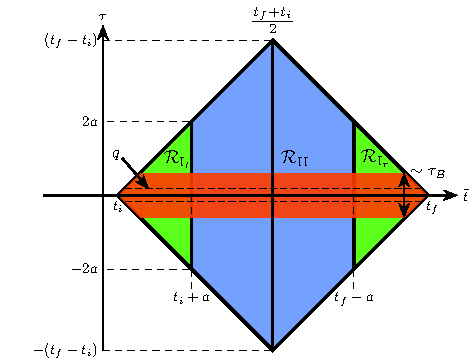
\includegraphics[width=.57\textwidth]{source/fig2.pdf}
\caption{本文の図\ref{fig1}に示した積分領域の、より詳細な模式図。部分領域 $\mathcal{R}_{\rm I}$ と $\mathcal{R}_{\rm II}$ を、それぞれ緑と青で示す。赤の領域は、FV 核 $k_r(\tau)$ が零でない台をもつ $(\tb,\tau)$ 平面の部分を表す。部分領域 $\mathcal{R}_{\rm II}$ では、$\tau$ の積分領域を無限大まで拡張し、本文と同様に扱うことができる。第 III 節では、$a$ によってパラメータ化された隅の領域 $\mathcal{R}_{{\rm I}_l}$ と $\mathcal{R}_{{\rm I}_r}$ の扱いを考える。試験関数 $x_{\tb}$ の、$a$ より短い時間尺度における変化は無視できるものと仮定する。}
\label{fig2}
\end{figure}

ここでは、本文の式\eqref{eq:decoh_action}で与えられるデコヒーレンス作用への端点項の寄与を、適切に扱うことを目指す。積分変数 $\tb$ と $\tau$ を用いると、この汎関数は
\be\label{eq:dec_func_end_terms}
	S_r[\Delta X] = \frac{1}{2}\iint_{\mathcal{R}_{\rm{I}} + \mathcal{R}_{\rm{II}}}d\tb\,d\tau\,k_r(\tau)\Delta X(\tb+\tau/2)\Delta X(\tb-\tau/2),
\ee
と書ける。ここで $\mathcal{R}_{\rm{I}/\rm{II}}$ は、図\ref{fig2}に緑と青で示した領域を定義する：
\begin{align*}
	&\mathcal{R}_{\rm I} = \mathcal{R}_{{\rm I}_l} \cup \mathcal{R}_{{\rm I}_r}\\
	&\qquad \mathcal{R}_{{\rm I}_l} = \{(\tb,\tau) :  t_i\leq \tb\leq t_i+a, \, -2(\tb-t_i)\leq\tau\leq 2(\tb-t_i)\} \\
	&\qquad \mathcal{R}_{{\rm I}_r} = \{(\tb,\tau) :  t_f-a\leq \tb\leq t_f, \, -2(t_f-\tb)\leq\tau\leq 2(t_f-\tb)\} \\
	&\text{および} \\
	&\mathcal{R}_{\rm II} = \mathcal{R}_{{\rm II}_l} \cup \mathcal{R}_{{\rm II}_r}\\
	&\qquad \mathcal{R}_{\rm {II}_l} = \{(\tb,\tau) : t_i+a\leq \tb\leq \frac{1}{2}(t_f+t_i), \, -2(\tb-t_i)\leq\tau\leq 2(\tb-t_i)\}  \\
	&\qquad \mathcal{R}_{\rm {II}_r} = \{(\tb,\tau) : \frac{1}{2}(t_f+t_i)\leq \tb\leq t_f-a, \, -2(t_f-\tb)\leq\tau\leq 2(t_f-\tb)\}.
\end{align*}
パラメータ $a$ は、端点 $t_i$ および $t_f$ に対する領域 $\mathcal{R}_{\rm II}$ の境界を定める。$a\gtrsim\tau_B$ を満たすように $a$ を固定すれば、赤の領域と比べて有意な寄与を拾うことがないため、$\mathcal{R}_{\rm II}$ における $\tau$ の積分範囲を実数直線全体まで拡張できる。また、この領域のパラメータ $q$ も、第 II 節と同様に任意に小さくできる。したがって、対応するデコヒーレンス汎関数は、$\tb$ の積分範囲を変更した、本文の式\eqref{eq:action}と同じ形をとる：
\begin{align}
	S^{\rm II}_r[\Delta X] &= \frac{1}{2}\int^{t_f-a}_{t_i+a}d\tb\int^{\infty}_{-\infty}d\tau\,k_r(\tau)\Delta X(\tb+\tau/2)\Delta X(\tb-\tau/2) \nonumber\\
		    &= \frac{2\eta}{\pi}\int^{t_f-a}_{t_i+a}d\tb\left[\frac{\pi}{\tau_B} \Delta X^2(\tb) + \int^{\infty}_0d\tau\,k^{(m)}_r(\tau)(\Delta X^2(\tb) - \Delta X(\tb+\tau/2)\Delta X(\tb-\tau/2))\right],
\end{align}
これは高温極限で
\be\label{eq:dec_func_II_htl}
	S^{\rm II}_r[\Delta X] \approx \frac{2\eta}{\tau_B}\int^{t_f-a}_{t_i+a}d\tb\,\Delta X(\tb)^2 + \frac{\eta\tau_B}{12}\int^{t_f-a}_{t_i+a}d\tb\,\Big(\Delta X'(\tb)^2 - \Delta X(\tb)\Delta X''(\tb)\Big).
\ee
となる。次に部分領域 $\mathcal{R}_{\rm I}$ を考えると、それぞれの隅の区分 $\mathcal{R}_{{\rm I}_l}$ および $\mathcal{R}_{{\rm I}_r}$ 内のデコヒーレンス作用は
\begin{subequations}
\begin{align}
    S^{{\rm I}_l}_r[\Delta X] &= \frac{1}{2}\int^{t_i+a}_{t_i}d\tb\int^{2(\tb-t_i)}_{-2(\tb-t_i)}d\tau\,k_r(\tau)\Delta X(\tb+\tau/2)\Delta X(\tb-\tau/2), \label{eq:decoh_action_l} \\
    S^{{\rm I}_r}_r[\Delta X] &= \frac{1}{2}\int^{t_f}_{t_f-a}d\tb\int^{2(t_f-\tb)}_{-2(t_f-\tb)}d\tau\,k_r(\tau)\Delta X(\tb+\tau/2)\Delta X(\tb-\tau/2). \label{eq:decoh_action_r}
\end{align}
\end{subequations}
で与えられる。各 $\tb$ 積分に対する、端点 $t_i$ および $t_f$ 近傍からの寄与を分離して、
\begin{subequations}
\begin{align}
    S^{{\rm I}_l}_r[x] &= \bar{S}^{{\rm I}_l}_r[x] + R^{{\rm I}_l}_r[x], \\
    S^{{\rm I}_r}_r[x] &= \bar{S}^{{\rm I}_r}_r[x] + R^{{\rm I}_r}_r[x],
\end{align}
\end{subequations}
とする。ここで、
\begin{subequations}
\begin{align}
    R^{{\rm I}_l}_r[x] &:= \frac{\eta}{\pi\tau_B}\int^{t^+_i}_{t_i}d\tb\int^{\frac{2(\tb - t_i)}{\tau_B}}_{\frac{-2(\tb - t_i)}{\tau_B}}ds\,F_{\Lambda}(s)x_{\tb}(s), \label{eq:R_left}\\
    R^{{\rm I}_r}_r[x] &:= \frac{\eta}{\pi\tau_B}\int^{t_f}_{t^-_f}d\tb\int^{\frac{2(t_f - \tb)}{\tau_B}}_{\frac{-2(t_f - \tb)}{\tau_B}}ds\,F_{\Lambda}(s)x_{\tb}(s),\label{eq:R_right}
\end{align}
\end{subequations}
は剰余項を定義する。左の隅の領域に対する剰余は、
\begin{align}
    \left|\int^{t^+_i}_{t_i} d\tb\int^{\frac{2(\tb - t_i)}{\tau_B}}_{-\frac{2(\tb - t_i)}{\tau_B}} ds\,F_{\Lambda}(s)x_{\tb}(s)\right| &\leq \int^{t^+_i}_{t_i} d\tb\int^{\frac{2(\tb - t_i)}{\tau_B}}_{-\frac{2(\tb - t_i)}{\tau_B}} ds\,|F_{\Lambda}(s)x_{\tb}(s)| \nonumber\\
    &\leq M_{\Lambda}\int^{t^+_i}_{t_i} d\tb\int^{\frac{2(\tb - t_i)}{\tau_B}}_{-\frac{2(\tb - t_i)}{\tau_B}}ds \nonumber\\
    &= 2M_{\Lambda}\frac{\delta t^2}{\tau_B},
\end{align}
から評価できる。ここで $M_{\Lambda} := \sup_{\tb,s\in\mathcal{R}_{{\rm I}_l}}|F_{\Lambda}(s)x_{\tb}(s)|$、$\delta t := t^+_i-t_i$ である。これより、
\be
    |R^{{\rm I}_l}_r| \leq \frac{2\eta M_{\Lambda}}{\pi}\frac{\delta t^2}{\tau^2_B},
\ee
が得られるので、$\delta t \ll \sqrt{\pi\tau^2_B/2\eta M_{\Lambda}}$ である限り、$R^{{\rm I}_l}_r[x]$ を小さくできる。同様の解析は $R^{{\rm I}_r}_r[x]$ にも適用できる。

次に作用汎関数 $\bar{S}^{{\rm I}_{l/r}}_r[\Delta X]$ に着目すると、式\eqref{eq:decoh_action_l}および\eqref{eq:decoh_action_r}の内側の積分は、第 II 節で述べたものと同じ手順に従って評価できる。その結果、
\begin{subequations}
\begin{align}
	\bar{S}^{{\rm I}_l}_r[\Delta X] &= \frac{2\eta}{\tau_B}\int^{t_i+a}_{t^+_i}d\tb\,\coth\left(\frac{2\pi(\tb-t_i)}{\tau_B}\right)\Delta X(\tb)^2 \nonumber\\
		      &\qquad + \frac{2\eta}{\pi}\int^{t_i+a}_{t^+_i}d\tb \int^{2(\tb-t_i)}_qd\tau\,k^{(m)}_r(\tau)\big(\Delta X^2(\tb) - \Delta X(\tb + \tau/2)\Delta X(\tb - \tau/2)\big), \label{eq:S_I_left}\\
	\bar{S}^{{\rm I}_r}_r[\Delta X] &= \frac{2\eta}{\tau_B}\int^{t^-_f}_{t_f-a}d\tb\,\coth\left(\frac{2\pi(t_f-\tb)}{\tau_B}\right)\Delta X(\tb)^2 \nonumber\\
		      &\qquad + \frac{2\eta}{\pi}\int^{t^-_f}_{t_f-a}d\tb \int^{2(t_f-\tb)}_qd\tau\,k^{(m)}_r(\tau)\big(\Delta X^2(\tb) - \Delta X(\tb + \tau/2)\Delta X(\tb - \tau/2)\big). \label{eq:S_I_right}
\end{align}
\end{subequations}
を得る。式\eqref{eq:T_lim}と異なり、$\tau$ 積分の極限 $q\rightarrow0$ を形式的にとることはできない点に注意されたい。$\lim_{\Lambda\rightarrow\infty}M_{\Lambda}=\infty$ であり、そのため剰余項 $R^{{\rm I}_{l/r}}_r[x]$ を適切に有界に保てなくなるからである。ただし、$q$ が十分小さい（あるいは $\Lambda$ が十分大きい）と仮定して、これらの積分の下限を近似的に零にすることはできる。

ここで高温極限を考える。式(\ref{eq:S_I_left})および(\ref{eq:S_I_right})の内側の項を $\tau$ の最低次まで展開すると、
\begin{subequations}
\begin{align}
	\bar{S}^{{\rm I}_l}_r[\Delta X] &\approx \Big(\dots\Big) + \frac{2\tau_B\eta}{\pi^2}\int^{t_i+a}_{t^+_i}d\tb\, B\left(\frac{2\pi(\tb-t_i)}{\tau_B}\right)\big(\Delta X'(\tb)^2 - \Delta X(\tb)\Delta X''(\tb)\big), \label{eq:S_I_l_htl} \\
	\bar{S}^{{\rm I}_r}_r[\Delta X] &\approx\Big(\dots\Big) + \frac{2\tau_B\eta}{\pi^2}\int^{t^-_f}_{t_f-a}d\tb\,B\left(\frac{2\pi(t_f-\tb)}{\tau_B}\right)\big(\Delta X'(\tb)^2 - \Delta X(\tb)\Delta X''(\tb)\big), \label{eq:S_I_r_htl}
\end{align}
\end{subequations}
となる。ここで $B(t)$ は、核 $k^{(m)}_r(\tau)$ の原始関数として
\be\label{eq:B}
	B\Big(\frac{\pi t}{\tau_B}\Big) := \frac{\pi}{\tau_B}\int^t_0d\tau\,k^{(m)}_r(\tau) = \int^{\frac{\pi t}{\tau_B}}_0dx\,x^2\csh^2x .
\ee
によって定義される。この積分の解析的な結果は、
\be\label{eq:B_scaled}
        B(t) = t\big[t - t\coth{t} + 2\ln(1-e^{-2t})\big] - {\rm Li}_2(e^{-2t}) + \frac{\pi^2}{6},
\ee
と求められる。ここで ${\rm Li}_s(t) = \sum^{\infty}_{k=1}\frac{t^k}{k^s}$ は多重対数関数である。

図\ref{fig3}には、$\tau_B$ のいくつかの値に対して積分 $B(\pi t/\tau_B)$ を示している。逆時間 $\tau^{-1}_B$ は、積分が漸近値に達する速さを決定する。したがって、$\tau_B$ が十分小さいとき、式(\ref{eq:S_I_left})の内側の積分は、境界 $t_i$ に近いものを除くほぼすべての $\tb$ の値について一定となる。$\tb$ が上限 $t_f$ に近づく場合の式(\ref{eq:S_I_right})の内側の積分についても、同じことが当てはまる。

\begin{figure}[t!]
\centering
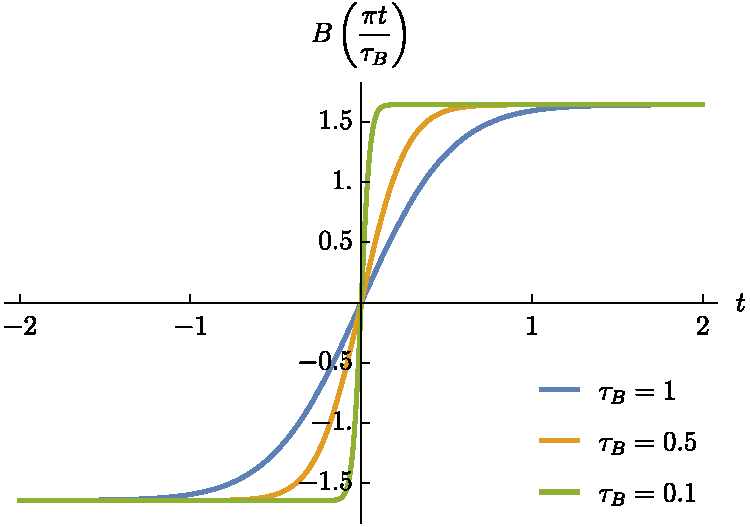
\includegraphics[width=.5\textwidth]{source/fig3.pdf}
\caption{\label{fig3} $t$ によって定まる上限を変化させたときの積分(\ref{eq:B})のプロット。$t\rightarrow\infty$ で値 $\frac{\pi^2}{6}$ に漸近する。式(\ref{eq:B_scaled})を参照。}
\end{figure}

この振る舞いは次のように定式化できる。$\mu(\tb)$ により測度を区分的に
\begin{align}
	d\mu(\tb) =
	\begin{cases}
		d\tb \qquad\qquad  & \tb\in(t_i+m, t_f-m\tau_B), \\
		\frac{6}{\pi^2}B\left(\frac{\tb-t_i}{\tau_B}\right)d\tb \qquad\qquad & \tb\in[t_i, t_i+m\tau_B], \\
		\frac{6}{\pi^2}B\left(\frac{t_f-\tb}{\tau_B}\right)d\tb \qquad\qquad  & \tb\in[t_f-m\tau_B, t_f],
	\end{cases}
\end{align}
と定義する。ここで $m\in\mathbb{R}^+$ は $B(m\tau_B/\pi)\sim \frac{\pi^2}{6}$ を満たすように選ぶ。このとき $\tau_B\rightarrow0$ とすると、$B(\pi t/\tau_B)$ が $\frac{\pi^2}{6}$ からずれる領域は、区間 $[t_i,t_f]$ の端点に限定される。これらの点の測度は零であるから、
\be\label{eq:int_measure}
	\lim_{\tau_B\rightarrow0}d\mu(\tb) =
	\begin{cases}
		d\tb \qquad &\tb\in(t_i,t_f), \\
		0, \qquad &\tb\in\{t_i,t_f\},
	\end{cases}
\ee
が成り立つ。$\mu(\tb)$ の極限での振る舞いを図\ref{fig4}に示す。

\begin{figure}[t!]
\centering
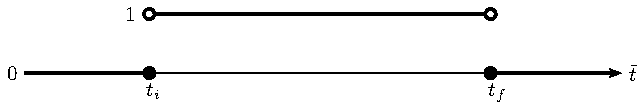
\includegraphics[width=.6\textwidth]{source/fig4.pdf}
\caption{\label{fig4} 高温極限において区間 $[t_i, t_f]$ に作用する積分測度 $d\mu(\tb)$。}
\end{figure}

式(\ref{eq:S_I_l_htl})および(\ref{eq:S_I_r_htl})はすでに $\tau_B$ が小さい極限で展開されているため、
\begin{align}\label{eq:dec_func_result}
	S_r[\Delta X] &= S^{\rm I}_r[\Delta X] + S^{\rm II}_r[\Delta X] \nonumber\\
	      &\approx \frac{2\eta}{\tau_B}\bigg[\int^{t_f-a}_{t_i+a}d\tb\,\Delta X(\tb)^2  \nonumber \\
	      &\qquad + \int^{t_i+a}_{t^+_i}d\tb\,\coth\left(\frac{2\pi(\tb-t_i)}{\tau_B}\right)\Delta X(\tb)^2 + \int^{t^-_f}_{t_f-a}d\tb\,\coth\left(\frac{2\pi(t_f-\tb)}{\tau_B}\right)\Delta X(\tb)^2\bigg] \nonumber\\
	      &\qquad + \frac{\eta\tau_B}{12}\int^{t_f}_{t_i}d\mu(\tb)\big(\Delta X'(\tb)^2 - \Delta X(\tb)X''(\tb)\big) + R^{{\rm I}_l}_r[\Delta X] + R^{{\rm I}_r}_r[\Delta X].
\end{align}
と書ける。さらに、同じ極限で
\begin{align*}
    &\lim_{\tau_B\rightarrow0}\coth\left(\frac{2\pi(\tb-t_i)}{\tau_B}\right) = 1 \qquad \tb\in(t_i,t_i+a), \\
    &\lim_{\tau_B\rightarrow0}\coth\left(\frac{2\pi(t_f-\tb)}{\tau_B}\right) = 1 \qquad \tb\in(t_f-a,t_f),
\end{align*}
に注意すると、式\eqref{eq:dec_func_result}の第1行と第2行も測度 $d\mu(\tb)$ を用いて次のように書ける：
\be
    S_r[\Delta X] \approx \int^{t_f}_{t_i}d\mu(\tb)\bigg[\frac{2\eta}{\tau_B}\Delta X^2(\tb) + \frac{\eta\tau_B}{12}\big(\Delta X'(\tb)^2 - \Delta X(\tb)\Delta X''(\tb)\big)\bigg] + R^{{\rm I}_l}_r[\Delta X] + R^{{\rm I}_r}_r[\Delta X].
\ee
したがって、デコヒーレンス汎関数 $S_r[\Delta X]$ の端点項を明示的に扱うことにより、剰余項を無視できるほど小さくできるならば、本文の式\eqref{eq:action}--\eqref{eq:decoh_action_1}と同様の結果が得られる。

\end{document}
